\providecommand{\topdir}{..}
\documentclass[../main.tex]{subfiles}


\begin{document}
	\chapter{Resonant X-ray Electric Field Intensity}\label{chap:07-res-XEFI}
	\section{Experimental Setup}

	\begin{figure}[H]
		\centering
		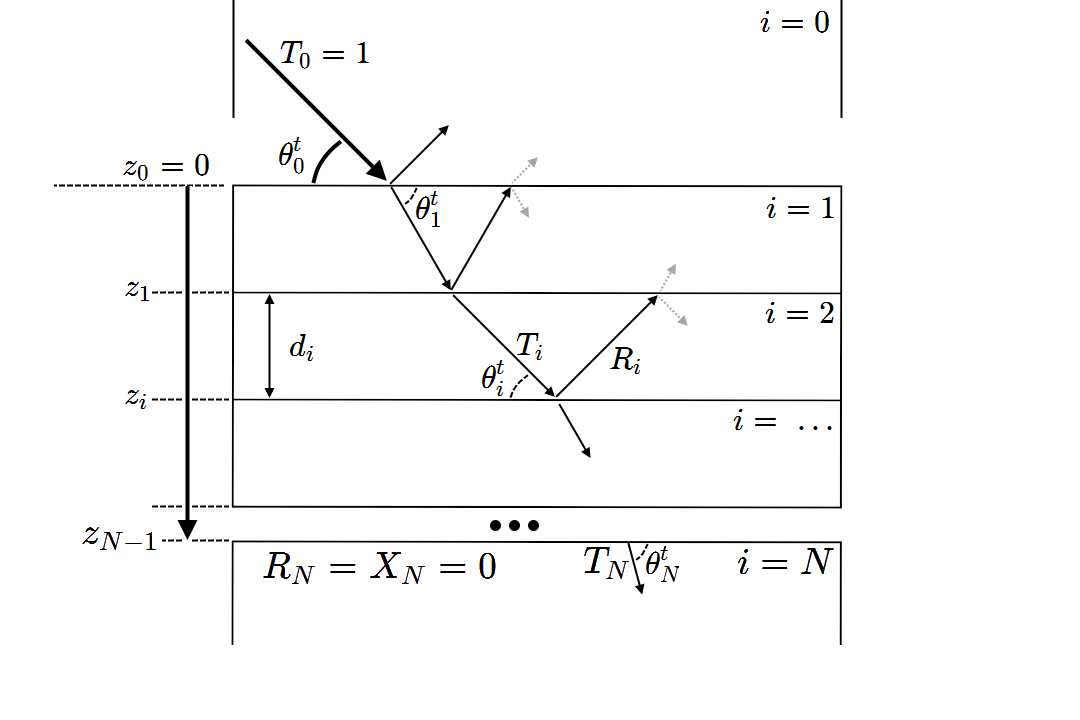
\includegraphics[width=0.8\textwidth]{resources/ch7/geometry.png}
		\caption{Experimental setup for measuring the X-ray electric field intensity. The X-ray beam is incident on a sample, and the reflected beam is analyzed to determine the electric field intensity.}
		\label{fig:experimental-setup}
	\end{figure}

	\subsection{Electric field}
	The total electric field of the X-ray beam in any given layer is given by the summation of two propogating waves.
	\begin{align}
		\vec{E_i}(\vec{r}) &= \vec{T_i}(\vec{r}) + \vec{R_i}(\vec{r})
	\end{align}
	where 
	\begin{align}
		\vec{T_i}(\vec{r}) &= T_i \cdot \exp\left(-\mathbf{i} \vec{k_{i}} \cdot \vec{r}\right) \\
		\vec{R_i}(\vec{r}) &= R_i \cdot \exp\left(+\mathbf{i} \vec{k_{i}} \cdot \vec{r}\right)
	\end{align}
	and $\vec{k_i}$ is the wavevector of the X-ray beam in layer $i$, at position $\vec{r}$.
	
	Here the transmission and reflection components represent the sum of all multiple-scattering events in the layer.
	The complex constants $T_i$ and $R_i$ result of the requirement for continuity of the electric field vector at the boundary - more specifically, through a recursive solution using the Frensel coefficients for each interface.

	Typically, especially for non-resonant X-ray scattering, the x-component wavevector $k_x$ is ignored and the attenuation is treated as negligible.

	\subsection{Angle of incidence and wavevector}
	For any radiation of wavelength $\lambda$, and incident angle $\theta_0$ coming from vacuum or a medium of complex refractive index $N$,
	the corresponding wavevector $\vec{k}$ is given by
	\begin{align}
		\vec{k_0} = \frac{2 \pi}{\lambda} \left( \cos(\theta_0) \hat{x} + \sin(\theta_0) \hat{z} \right)
	\end{align}
	
	As the X-ray propogates through the sample, the dielectric constant modifies the (now complex) angle of incidence and the 
	complex wavevector, as per Snell's law (for grazing incidence).

	\begin{align}
		\theta_i &= \arccos\left(\frac{\cos\left(\theta_0\right) \times N_0}{N_i}\right)\\
		\vec{k_i} &= |\vec{k_0}| \left( \cos(\theta_i) \hat{x} + \sin(\theta_i) \hat{z} \right)
	\end{align}	

	\subsubsection{Critical angle}
	For any given refractive index $N_i < N_0$ \footnote{This is usually the case for X-rays where $N_i = 1 - \delta_i + \mathbf{i}\beta_i$}, the critical angle occurs when $\cos\left(\theta_0\right) < \frac{N_i}{N_0}$.
	In the case where $N_0 \approxeq 1$ is air/vacuum, this critical angle corresponds to
	\begin{align}
		\theta_{0} &= \sqrt{2 \delta_i}
	\end{align}

	\section{Interface Calculation}
	To calculate the effect of refraction and reflection at each interface, a boundary condition is applied that the tangential component of the electric field must be continuous across the interface (both in $\hat{x}$ and $\hat{y}$ directions). This requires knowledge of the polarisation of the X-ray beam, as well as the refractive index of the medium.

	\subsection{Polarisation Dependence}
	An x-ray can be S-polarised (parallel to the planar surface, i.e. in the $\hat{y}$ or $\hat{x}$ direction) or P-polarised (parallel to the planar normal, i.e. in the $\hat{z}$ plane). These are also known as transverse electric (TE) and transverse magnetic (TM) polarisations, respectively.

	Usually, the polarisation angle $\alpha$ can be defined as the angle between the electric field vector and the plane of incidence, with $\alpha = 0$ for S-polarised waves and $\alpha = \frac{\pi}{2}$ for P-polarised waves. Then the perpendicular and parallel components of the electric field vector can be defined as
	\begin{align}
		E_{i, \perp} &= E_i \cos(\alpha) \\
		E_{i, \parallel} &= E_i \sin(\alpha)
	\end{align}

	In the context of grazing incidence experiments, the X-ray beam is typically highly aligned and polarised. It will be routine to perform measurements with both S- and P-polarised X-rays.

	\subsection{Frensel Coefficients}
	Frensel coefficients describe the amplitude of reflected and transmitted waves at an interface between two media with different refractive indices. For S-polarised waves, the Frensel coefficients are given by
	\begin{align}
		t_{s, i} &= \frac{2 k_{i, z}}{k_{i, z} + k_{t, z}} \\
		r_{s, i} &= \frac{k_{i, z} - k_{t, z}}{k_{i,z} + k_{t,z}} = t_{s,i} - 1
	\end{align}
	For P-polarised waves, the Fresnel coefficients are given by
	\begin{align}
		t_{p, i} &= \frac{2 k_{i, z}}{n^2 k_{i, z} + k_{t, z}} \\
		r_{p, i} &= \frac{n^2 k_{t, z} - k_{i, z}}{n^2 k_{t,z} + k_{i,z}}
	\end{align}
	At resonance, the refractive index $n$ can be modified by a significant amount. Consider the imaginary component in Polystyrene (CH) at the carbon K edge changing magnitude from 1e-4 to 6e-3. For P3MEEET (C11H16O3S) at the resonant sulfur K edge, the magnitude changes from 9e-7 to 5.7e-6.

	\section{Taylor Series Derivation}
	Following the derivation of Borne \& Wolf (1985) and Savakhin et al. (2020).
	
	The total electric field is the sum of many reflections.
	\begin{align}
		E = E_1 + E_2 + E_3 + ... + E_N
	\end{align}
	
	As we 

	
	\ifSubfilesClassLoaded{
		\printbibliography{}
		\printglossaries
	}{} % we have no 'else' action
	
\end{document}